%Semiblind Multiuser Detection for synchronous CDMA. This presentation scheduled on March 19th, 2003

\documentclass[20pt,landscape]{foils}
\usepackage[pdftex]{color}
\usepackage[pdftex]{graphicx}
\usepackage[pdftex]{geometry}
\geometry{headsep=2ex,hscale=0.9} \pdfpagewidth=11in
\pdfpageheight=8.5in

\setlength{\footskip}{0.0in} \setlength{\textheight}{8.0in}

\usepackage{background}
\usepackage{pp4slide}
%\usepackage{pdfscreen}

\newcommand{\br}{{\mathbf r}}
\newcommand{\bA}{{\mathbf A}}
\newcommand{\ba}{{\bf a}}
\newcommand{\bb}{{\bf b}}
\newcommand{\bc}{{\bf c}}
\newcommand{\bC}{{\bf C}}
\newcommand{\bd}{{\bf d}}
\newcommand{\be}{{\bf e}}
\newcommand{\bh}{{\bf h}}
\newcommand{\bbm}{{\bf m}}
\newcommand{\bt}{{\bf t}}
\newcommand{\bs}{{\bf s}}
\newcommand{\bn}{{\bf n}}
\newcommand{\bu}{{\bf u}}
\newcommand{\bv}{{\bf v}}
\newcommand{\bw}{{\bf w}}
\newcommand{\bx}{{\bf x}}
\newcommand{\bz}{{\bf z}}
\newcommand{\by}{{\bf y}}
\newcommand{\bbf}{{\bf f}}
\newcommand{\bF}{{\bf F}}
\newcommand{\bH}{{\bf H}}
\newcommand{\bL}{{\bf L}}
\newcommand{\bM}{{\bf M}}
\newcommand{\bN}{{\bf N}}
\newcommand{\bbP}{{\bf P}}
\newcommand{\bQ}{{\bf Q}}
\newcommand{\bS}{{\bf S}}
\newcommand{\bT}{{\bf T}}
\newcommand{\bD}{{\bf D}}
\newcommand{\bX}{{\bf X}}
\newcommand{\bY}{{\bf Y}}
\newcommand{\bP}{{\bf P}}
\newcommand{\bI}{{\bf I}}
\newcommand{\bR}{{\bf R}}
\newcommand{\bU}{{\bf U}}
\newcommand{\bV}{{\bf V}}
\newcommand{\bW}{{\bf W}}
\newcommand{\bJ}{{\bf J}}
\newcommand{\bB}{{\bf B}}
\newcommand{\bzero}{{\bf 0}}
\newcommand{\bgamma}{{\mbox {\boldmath $\gamma$}}}
\newcommand{\btheta}{{\mbox {\boldmath $\theta$}}}
\newcommand{\bLambda}{{\mbox {\boldmath $\Lambda$}}}
\newcommand{\bPsi}{{\mbox {\boldmath $\Psi$}}}
\newcommand{\bPhi}{{\mbox {\boldmath $\Phi$}}}
\newcommand{\bcS}{{\mbox {\boldmath ${\cal S}$}}}
\newcommand{\bcH}{{\mbox {\boldmath ${\cal H}$}}}
\newcommand{\bcI}{{\mbox {\boldmath ${\cal I}$}}}
\newcommand{\bcP}{{\mbox {\boldmath ${\cal P}$}}}
\newcommand{\bcQ}{{\mbox {\boldmath ${\cal Q}$}}}
\newcommand{\bcR}{{\mbox {\boldmath ${\cal R}$}}}
\newcommand{\bcB}{{\mbox {\boldmath ${\cal B}$}}}

\zerolistvertdimens

\begin{document}
\raggedright \color{black}
\definecolor{bgcolor}{rgb}{1,1,1}
\pagecolor{bgcolor} % set background color
\definecolor{bgblue}{rgb}{0.04,0.37,0.59}
\vpagecolor{bgblue}


\foilhead{\LARGE Semi-Blind Decorrelating Multiuser Detection for
Synchronous CDMA}

\begin{center}
\vspace{.3in}
{\bf Shu Wang, James Caffery, Jr. and Hanhong Shen}  \\
{\it \vspace{0.9in} Wireless System Research Laboratory \\
\vspace{0.2in} Dept. of Elec. \& Comp. Engin. \& Comp. Scien.
\\ University of Cincinnati\\
{\bf WCNC 2002 \\ New Orleans, Los}}
\end{center}

\foilhead[-.4in]{Introduction}
\begin{itemize}
\item CDMA techniques have attracted attention for their spectral
efficiency, interference resistance and flexible traffic control.
\item MAI is the dominant impairment for CDMA systems and exits
even with perfect power control.
%\item Multiuser detection describes method that minimize the effects of
%MAI and mitigate the near-far problem.
%\item Interference cancellation provides a promising alternative
%to the conventional or optimum detectors in multiuser detection.
\item Multiuser detection promising approach to mitigate MAI:
classic/non-blind multiuser detection and blind multiuser
detection

\item With exploring a new data model and the trade-off between
classic multiuser detection and blind multiuser detection, we
propose semi-blind decorrelating multiuser detection.
 \begin{itemize}
 \item Least squares semi-blind decorrelating multiuser detection (LS-DD)
 \item Total least squares semi-blind decorrelating multiuser detection (TLS-DD)
 \item Mixed LS/TLS  semi-blind decorrelating multiuser detection (MLS-DD)
 \end{itemize}
\end{itemize}

%%
\foilhead[-.5in]{Data Model}
\begin{itemize}
\zerolistvertdimens \item Consider a synchronous CDMA system with
$L$ chips per bit ($T_{b}=L T_{c}$). \item Received signal, after
chip-matched filter followed by chip-rate sampling: \vspace{-.2in}
$$
\br = \sum_{k=1}^{K} A_{k} b_{k} \bs_{k} + \bn \; = \; \bS \bA \bb
+ \bn
$$
where $\bA={\sf diag}\left\{ A_{1} \; A_{2} \; \ldots \; A_{K}
\right\}$, $\bS=\left[ \bs_{1} \; \bs_{2} \; \ldots \; \bs_{K}
\right]$ and $\bb = \left[ b_{1} \; b_{2} \; \ldots \; b_{K}
\right]^{T}$ with $b_{i} \in \left\{ +1,-1 \right\}$. \item Linear
multiuser detectors can be written in the form  \vspace{-.2in}
$$
\bb = {\sf sgn} \left\{ \bW \br \right\} \vspace{-.2in}
$$
or for the $k$th user {\color{htext} $b_{k} = {\sf sgn} \left\{
\bw^{T}_{k} \br \right\}$} where $\bw_{k}^{T}$ is the $k$th row of
$\bW$. \item We consider detection of user 1's data only. \item
Maintain the restriction that $L>K$.
\end{itemize}

\foilhead[-.5in]{New Data Model w.r.t. User 1 -- I}
\begin{itemize}

\item In terms of user 1, a new semi-blind signature matrix $\bcS$
is constructed by

$$
\begin{array}{rcl}
\bcS&=&[\matrix{A_1\bs_1&\br_{1}&\br_{2}&\ldots&\br_{M-1}}]\\
 &=&\bS\bA\left[\matrix{\be_1 & \bD }\right]+ \bN\\
 &=&\bS\bA\bB + \bN
\end{array}$$

\noindent where $\bB=\left[\matrix{1& \bar{\bd}^{T} \cr
\mathbf{0}& \tilde{\bD} }\right]=\left[\matrix{\bc^{T} \cr
\matrix{\mathbf{0}& \tilde{\bD}} }\right]$.

\item The relationship between $\br$ and $\bcS$ is
$$
\br=\bcS\bd + \bf z
$$
\noindent where $\bd$ is named the detection vector.
$$\bd = \bB^{+}\bb =
\left[\matrix{1&\bar{\bd}^T\cr\mathbf{0}&\tilde{\bD}}
\right]^{+}\left[\matrix{b_1\cr\tilde{\bb}}\right] $$

\end{itemize}


\foilhead[-.5in]{New Data Model w.r.t. User 1  -- II  }
\begin{itemize}
\item $\bN$ is a noise matrix of the form, $\bN=[\mathbf{0}\
\tilde{\bN}]$. $\bf z$ is the new noise vector defined as ${\bf
z}=\bn-\bN\bB^{+}\bb$.



\item The bit sent by the first user, $b_1$, during the time
interval $t\in[(n-1)T,\ nT]$ can be estimated as

$$
b_1 =  \bc^T\bd
$$

\noindent where $\bc=[\matrix{1&\bar{\bd}^T}]^T$ and
$\bd=\left[\matrix{d_1&\tilde{\bd}} \right]^T$.

\item Now, the semi-blind multiuser detection problem becomes how
to estimate $\bd$.
\end{itemize}

%%
\foilhead{Least-Square Semi-blind Multiuser Detection (LS-DD)}
\begin{itemize}
\item The LS estimation problem is

$$
\matrix{\bd_{\rm
LS}&=&\min\limits_{\bx}\left\|\bcS\bx-\br\right\|_2}
$$

\item The LS solution is
$$\bd_{\rm LS}=\bcS^+\br$$
\noindent and the bit sent by the first user, $b_1$, in the $n$th
signaling interval is detected with
$$
\begin{array}{rcl}
\hat{b}^{\rm LS}_{1}&=&\mbox{sgn}\{\bw_{\rm LS}^{T}\br\}\\
 &=&\mbox{sgn}\left\{b_1+\bc^T\bcS^+\tilde{\bn}\right\} \enspace .
\end{array}
$$

\item In LS estimation, it assumes that $\bcS$ is error-free.
However, this assumption is not entirely accurate according since
there is a noise term, $\bN$.

\end{itemize}

%%
\foilhead{Total Least-Square Semi-blind Multiuser Detection
(TLS-DD)}
\begin{itemize}
\item $\br$ can also be expressed as $\br=\hat{\bcS}\bd + \bn$,
where  $\hat{\bcS}=\bcS-\bN=\bS\bA\bB$.
\item  The LS problem can
then be transformed into the following TLS problem:
$$
\begin{array}{rcl}
\bd_{\rm TLS}&=&\matrix{\min\limits_{\bar{\bcS},\
\bx}\left\|\left[ \matrix{\bcS&\br} \right] - \left[
\matrix{\bar{\bcS}& \bar{\bcS}\bx}\right]\right\|_2}
\end{array}.
$$

\item The TLS solution is $$\bd_{\rm TLS}=
\left(\bcS^T\bcS-\sigma_{K+1}^2\bI\right)^{-1}\bcS^T\br$$

\noindent and the $n$th bit sent by the first user, $b_1$, can be
detected with
$$\begin{array}{rcl}
\hat{b}^{\rm TLS}_{1}&=&\mbox{sgn}\{\bw_{\rm TLS}^T\br\}\\
 &=&\mbox{sgn}\left\{ \bc^T\left(\bcS^T\bcS-\sigma_{K+1}^2\bI\right)^{-1}
 \bcS^T\br\right\} \enspace .
% &=&\mbox{sgn}\{b_n^1+[\matrix{A_1^{-1}&\bar{\bd}^T}]\bcS^+\tilde{\bn}\}
\end{array}
$$
\end{itemize}


%%
\foilhead{Mixed LS/TLS Semi-blind Multiuser Detection (MLS-DD) I}
\begin{itemize}
\item In the LS problem, it assumed the semi-blind signature
matrix $\bcS$ is error-free. Again, this assumption is not
completely accurate.

\item In the TLS problem, it assumed that in each column of the
semi-blind signature matrix, $\bcS$, some noise or error exists.
This assumption also is not complete.

\item Hence, to maximize the estimation accuracy of the detection
vector $\bd$, it is natural to require that the corresponding
columns of $\bcS$ be unperturbed since they are known exactly. The
estimation problem becomes the following MLS problem.

$$
\begin{array}{rcl}
\bd_{\rm MLS}&=&\matrix{\min\limits_{\bar{\bcS},\
\bx}\left\|\left[\matrix{\tilde{\bcS}&\br}\right]-\left[\matrix{\bar{\bcS}&[A_1\bs_1\
 \bar{\bcS}]\bx}\right]\right\|_{2} }
\end{array}
$$
\end{itemize}


%%
\foilhead{Mixed LS/TLS Semi-blind Multiuser Detection (MLS-DD) II}
\begin{itemize}
\item The MLS solution is given by

$$
\begin{array}{rcl} \bd_{\rm
MLS}&=&\left(\bcS^T\bcS-\sigma^2\left[\matrix{0&\mathbf{0}\cr\mathbf{0}&\mathbf{I}_{M-1}}\right]\right)^{-1}\bcS^T\br
\end{array}.
$$

\noindent and the bit sent by the first user, $b_1$, can be
detected with
$$
\begin{array}{l}
\hat{b}^{\rm MLS}_{1}=\mbox{sgn}\{\bw_{\rm MLS}^{T}\br\}\\
 =\mbox{sgn}\left\{\bc^T\left(\bcS^T\bcS-\sigma^2\left[\matrix{0&\mathbf{0}\cr\mathbf{0}&\mathbf{I}_{M-1}}\right]\right)^{-1}\bcS^T\br\right\}.
\end{array}
$$
\end{itemize}


\foilhead{Performance Analysis I}

\begin{itemize}

\item When $\bN=\mathbf{0}$, the proposed LS-DD and the classic
decorrelating detector share the same signature space and

$$
\bw_{\rm LS} = A_k^{-1}\bw_{\rm DD} \enspace . \label{wN0}
$$

Hence, they share the same performance for user 1, too.

\item It is straightforward to develop the following relationship
between the estimation errors of $b_1$ and $\bd$:
$$ \Delta b_1\leq \|\Delta\bd\|_1 $$

\noindent where $\Delta b_1=\hat{b}_1-b_1$,
$\Delta\bd=\hat{\bd}-\bd$ and $\|{\bf m}\|_1$ denotes the 1-norm
of the vector $\bf m$ .

\end{itemize}


\foilhead{Performance Analysis II}

\begin{itemize}

\item The mean of the semi-blind noise item $ \bz $ is
$$
\begin{array}{rcccl}
\mu&=&E\{\bz\}&=&0 \enspace .
\end{array}
$$

\item The variance of the semi-blind noise item $\bz$ satisfies
the following inequality
$$
\begin{array}{rcl}
\max\{var\{\bz\}\}&=&\max\{E\{(\bz-\mu)^2\}\}\\
&\leq&\sigma^2+(K-1)\|\tilde{\bD}^+\|_2^2\sigma_N^2
\end{array}
$$
where $\max\{{\bf m}\}$ denotes the maximum item in the vector
$\bf m$ and $\sigma_N^2$ is the power of the noise item $\bN$ in
the semi-blind signature matrix $\bcS$.

\end{itemize}


\foilhead{Computer Simulations I}
\begin{figure}
\center{
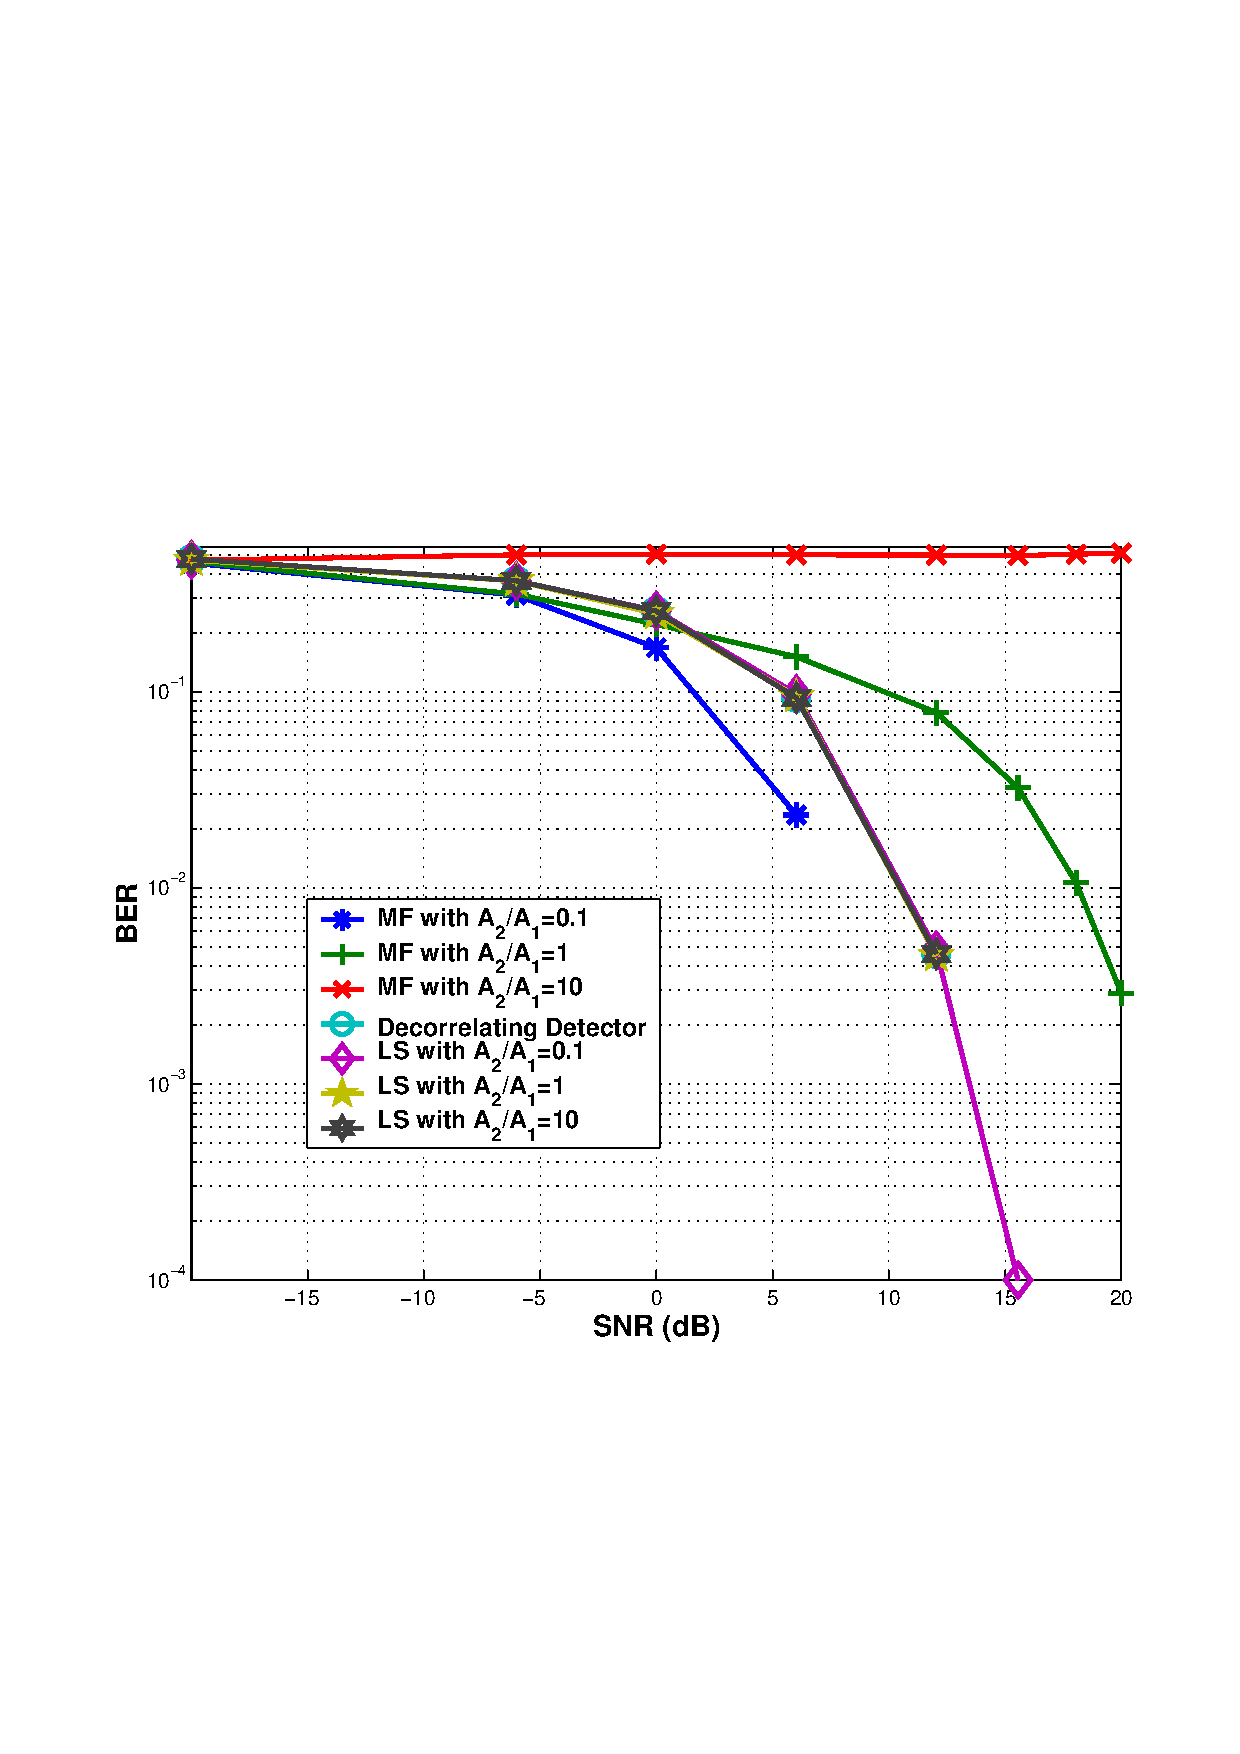
\includegraphics[width=6in]{SynchSemiBlindBER_LS0.pdf}}
\end{figure}
\center{BER comparison of the single-user matched filter,
decorrelating detector, and the LS semi-blind detector for the
first user in a two user system with $\rho=0.75$.}


\foilhead{Computer Simulations II}
\begin{figure}
\center{
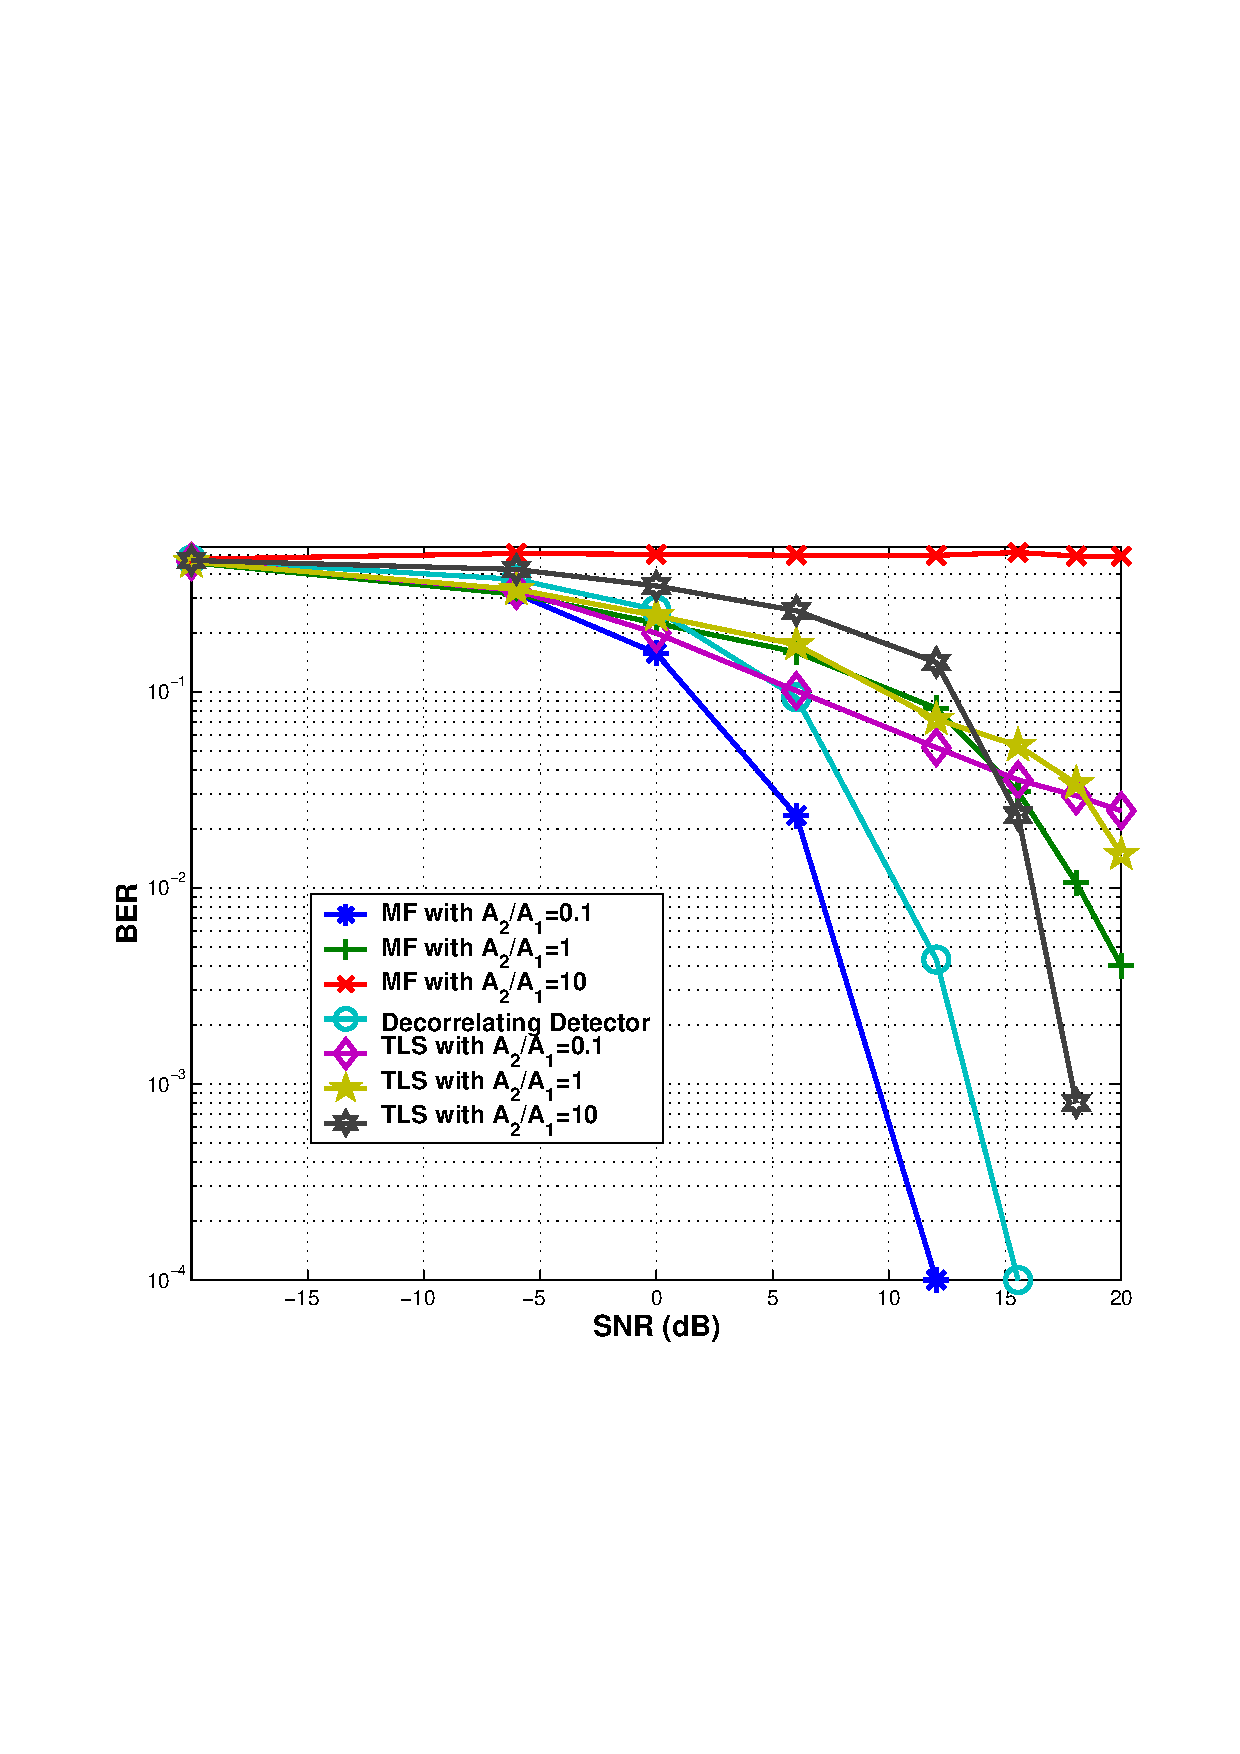
\includegraphics[width=6in]{SynchSemiBlindBER_TLS.pdf}}
\end{figure}
\center{BER comparison of the single-user matched filter,
decorrelating detector, and the TLS semi-blind detector for the
first user in a two user system with $\rho=0.75$.}

\foilhead{Computer Simulations III}
\begin{figure}
\center{
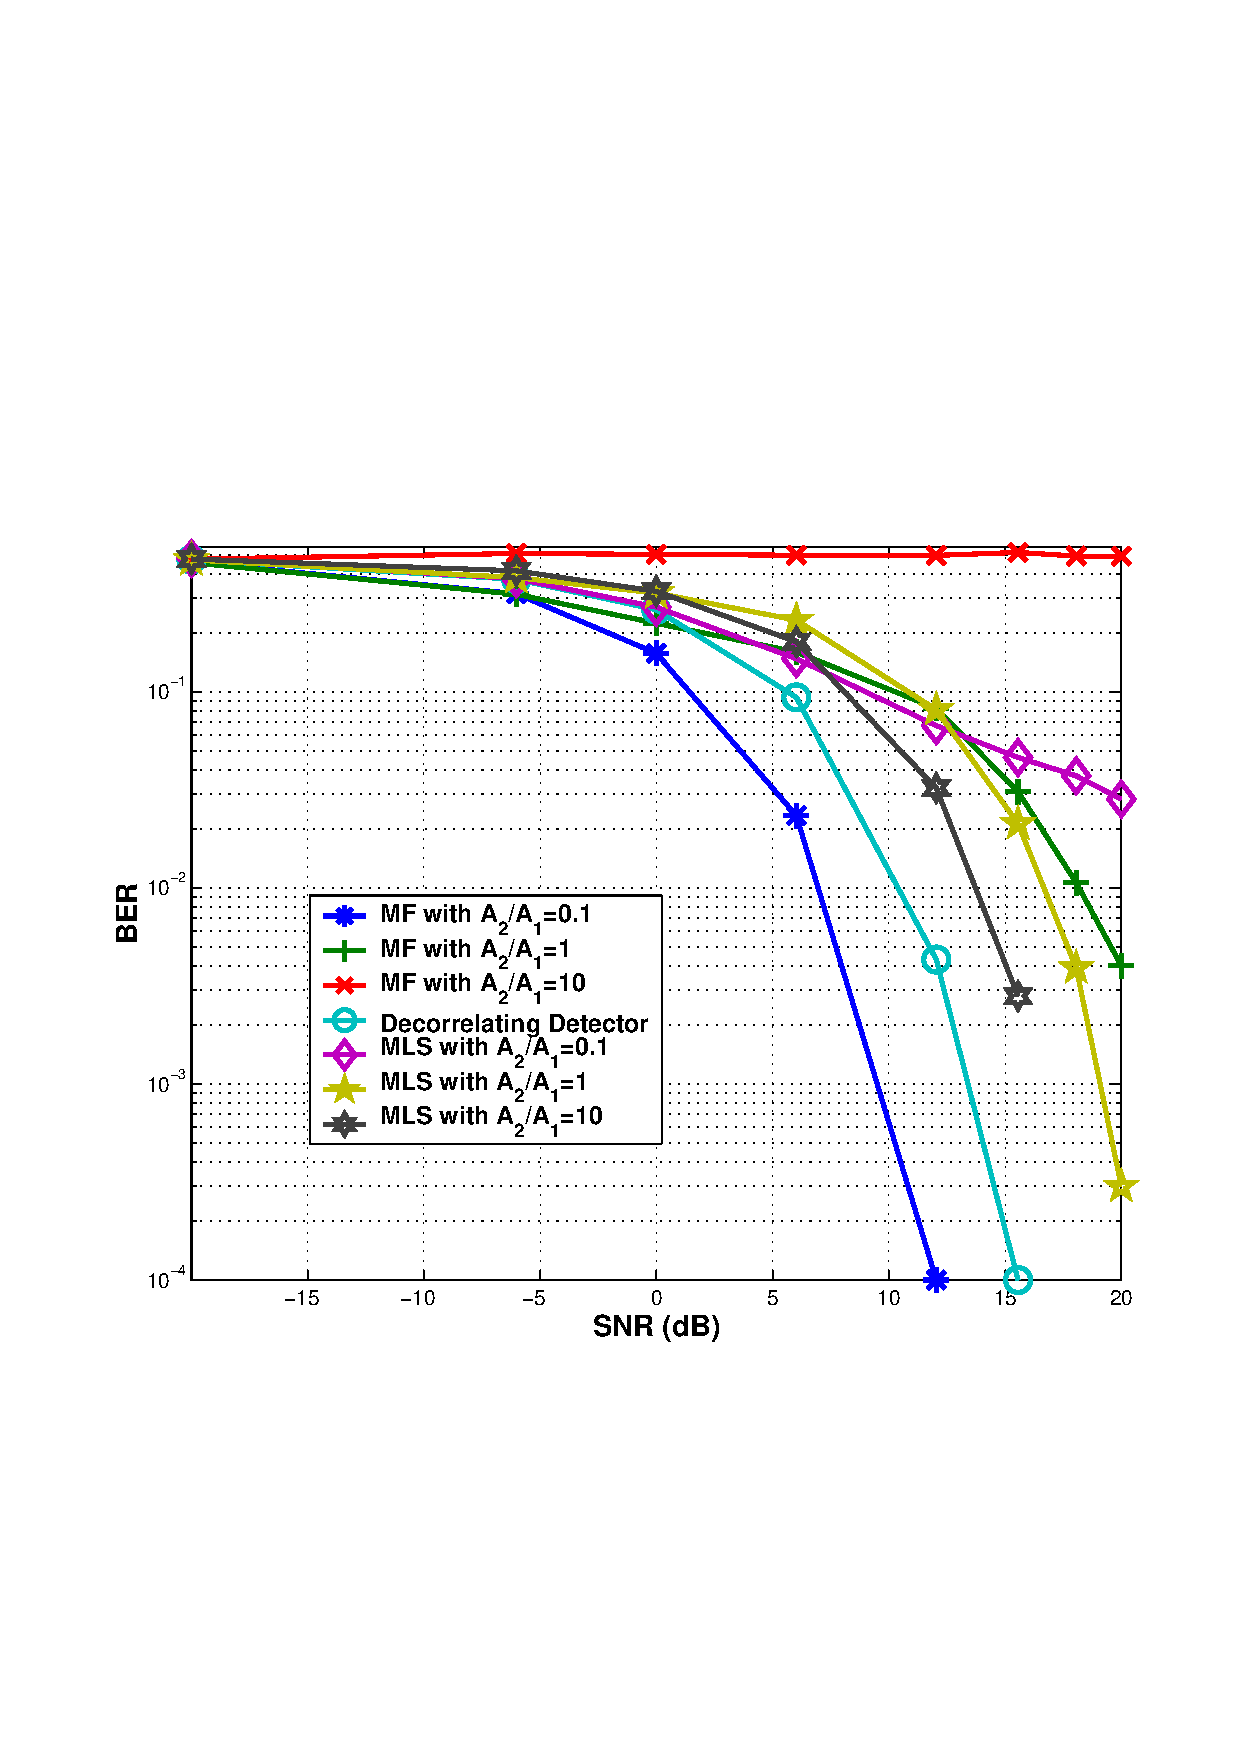
\includegraphics[width=6in]{SynchSemiBlindBER_MLS.pdf}}
\end{figure}
\center{BER comparison of the single-user matched filter,
decorrelating detector, and the MLS semi-blind detector for the
first user in a two user system with $\rho=0.75$.}


\foilhead{Computer Simulations IV}
\begin{figure}
\center{
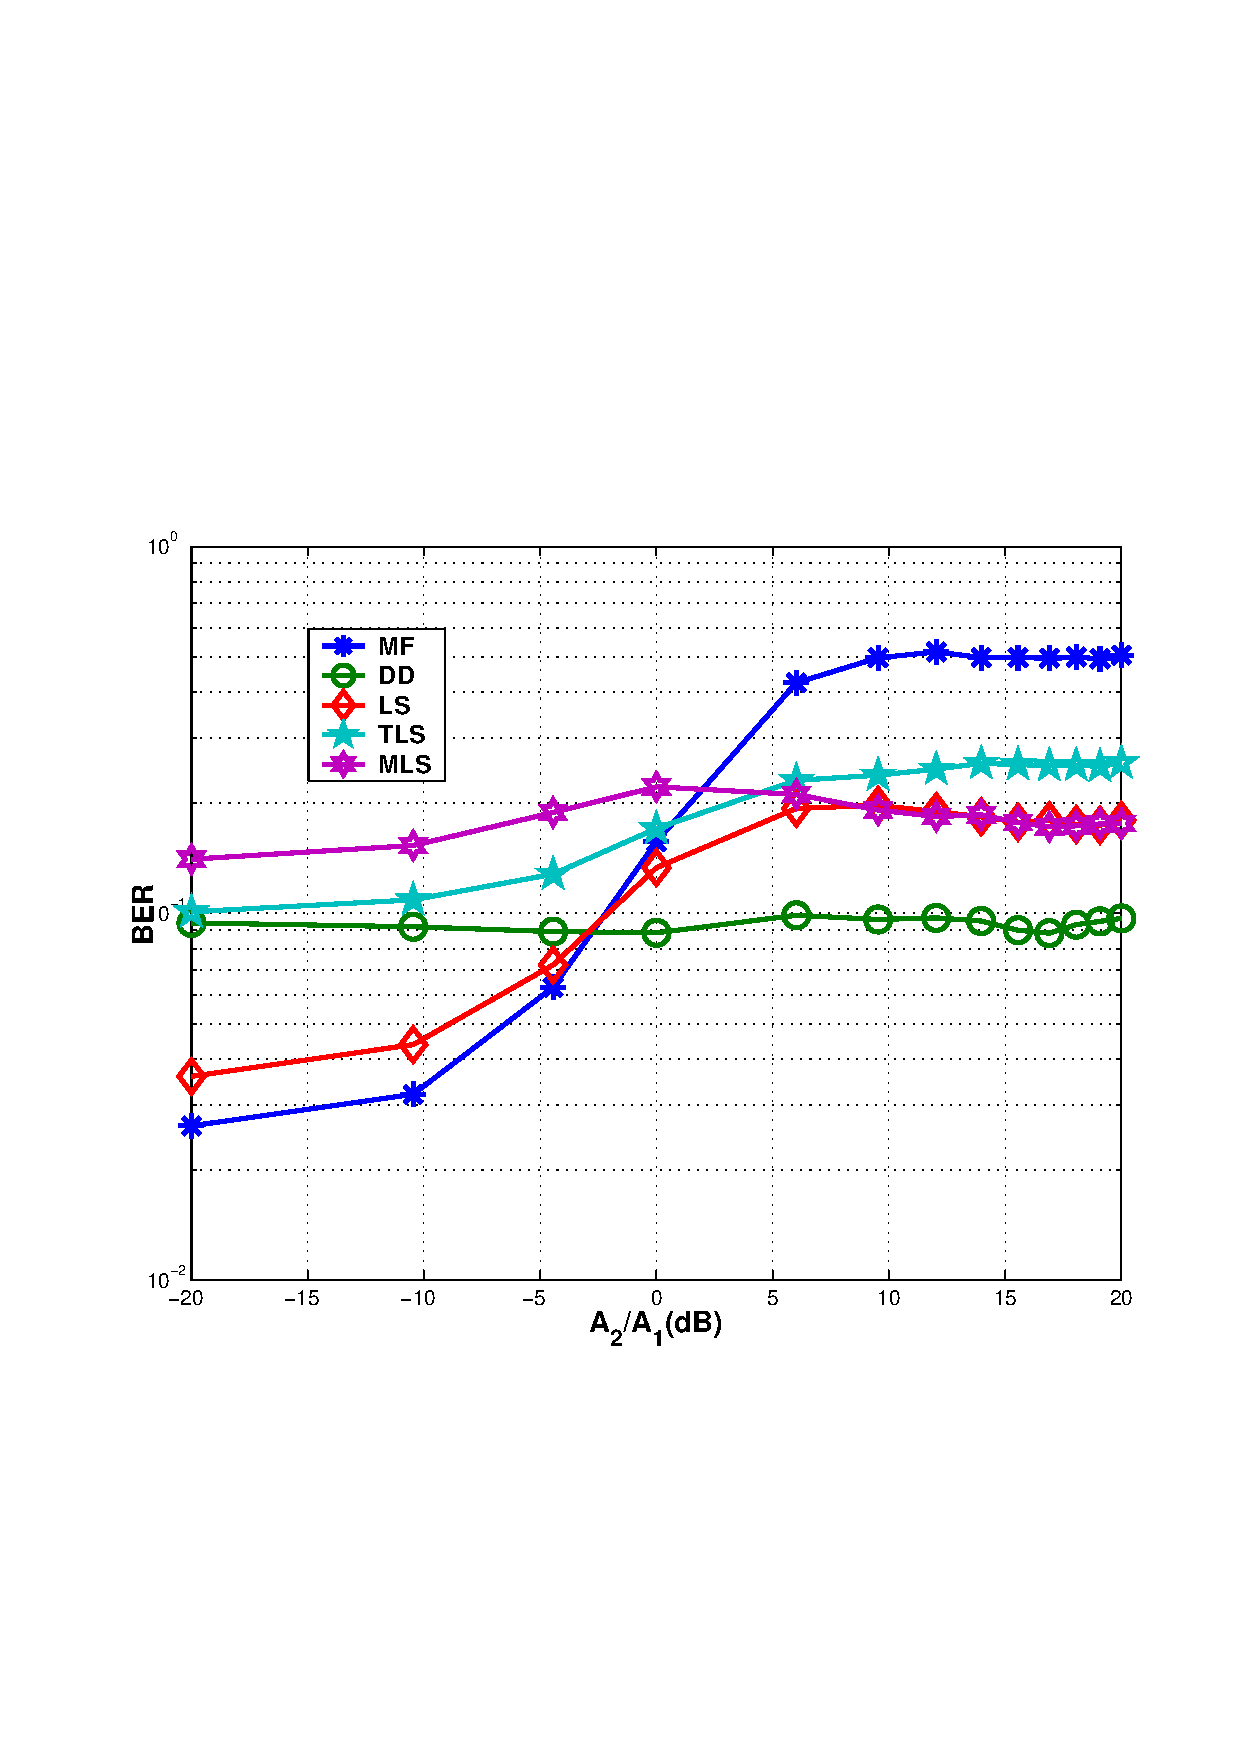
\includegraphics[width=6in]{SynchSemiBlindNFR.pdf}}
\end{figure}
\center{Near-far resistance comparison of the single-user matched
filter, decorrelating detector, and the LS, TLS and MLS semi-blind
detectors for the first user in a two user system with $\rho=0.75$
and $SNR=6dB$.}


%%
\foilhead{Conclusion \& Future Directions}
\begin{itemize}
\item Multiuser precoding provides another alternative to solve
the near-far problem in multiuser systems.

\item With linear system theory, it can be shown that many linear
multiuser precoders and detectors can achieve the same
performance.

\item With considering the input information bits, nonlinear
multiuser precoding can be developed to further enhance system
performance.

\item Additional performance enhancement may be achievable by
jointly optimizing transmitter multiuser precoding and adaptive
receivers/transmitters.

\item For unknown or time-variable channels, adaptive multiuser
precoding with feedback from receivers  amd multiuser precoding
with channel coding can be interesting topics.

\end{itemize}

\end{document}
